\chapter{Analisis dan Rancangan Klasifikasi Teks Berbahasa Indonesia Menggunakan \textit{Multilingual Language Model}}

Bab ini berisi analisis dan rancangan berkaitan dengan studi literatur pada bab sebelumnya. Oleh karena itu, bab ini terdiri dari analisis permasalahan dan rancangan solusi.

\section{Analisis Permasalahan}
	Subbab ini berisi analisis dari dua permasalahan klasifikasi teks yang akan diselesaikan, yaitu analisis sentimen dan klasifikasi ujaran kebencian.

	\subsection{Analisis Permasalahan Analisis Sentimen}
	Pada penelitian ini, digunakan dua buah dataset. Dataset pertama, dirujuk sebagai dataset A, adalah dataset yang sama dengan penelitian \parencite{FarhanKhodra2017}. Dataset tersebut merupakan ulasan-ulasan dari situs TripAdvisor yang kemudian dilabeli positif untuk nilai 3-5 dan negatif untuk nilai 1-2. Dataset kedua, dirujuk sebagai dataset B,  dan dataset dari Prosa.ai \parencite{CrisdayantiPurwarianti2019}. Dataset tersebut berupa kumpulan teks Twitter, Zomato, Facebook, Instagram, Qraved yang sudah dianotasi oleh annotator profesional. Setiap ulasan, yang terdiri dari satu sampai tiga kalimat, dapat memiliki frasa sentimen di awal, di tengah, dan di akhir dokumen. Berikut contoh ulasan yang berlabel negatif.

	“Kemaren sengaja coba makan di marugame udon karena istri suka banget sama udon. jadi pesan lah yang kuah kaldu ayam, dan anak saya minta gorengan kroket. saya kira kuahnya langsung dari pancinya harusnya panas, tapi ternyata cuman hangat, yah kecewa juga sih, gorengannya juga sama udah dingin” 

	Dapat dilihat dari paragraf di atas, kalimat awal pada paragraf tersebut tidak mengandung sentimen apapun. Frasa sentimen baru ditemui di akhir paragraf. Berikut contoh ulasan yang berlabel positif.

	“berlokasi di pusat jakarta.. sangat mudah mengakses ke berbagai tempat strategis dan keramaian. hotel sangat bersih, pelayanan ramah dan makanan sesuai lidah indonesia atau western. sangat direkomendasikan.”

	Dapat dilihat dari paragraf di atas, frasa sentimen positif sudah langsung diutarakan pada awal paragraf. Tetapi tidak semua ulasan memiliki satu sentimen saja. Berikut ini adalah salah satu contoh ulasan pada dataset yang mengandung frasa sentimen negatif dan positif disaat bersamaan. 

	“Kelihatan dari luar memang menarik tempatnya. Suasananya juga cozy. Saat makan siang juga ramai pengunjung. AC tidak berasa, jadi lumayan panas di dalam. Memesan nasi dengan irisan slice pork belly, nasinya tanpa bumbu apa- apa jadi kering banget, irisan pork belly nya dominan lemak dan minyak. Kita dapat 6 slice, tapi sesudah makan slice ke 3, rasanya tidak sanggup lagi karena merasa eneg dengan lemak pork belly nya.”

	Dapat dilihat dari paragraf di atas, tiga kalimat pertama menunjukkan opini positif sedangkan 3 kalimat terakhir menunjukkan opini negatif. Tetapi berdasarkan analisis keseluruhan, dapat dilihat bahwa ulasan tersebut bersentimen negatif.

	Penelitian terkait oleh \parencite{FarhanKhodra2017} dan \parencite{CrisdayantiPurwarianti2019} sudah mengekplorasi berbagai jenis representasi dokumen dan topologi untuk menyelesaikan analisis sentimen level dokumen pada data tersebut. Meski sudah mendapatkan hasil, penelitian terkait sebelumnya belum mengeksplorasi penggunaan \textit{language model} dalam bentuk apapun, terlebih lagi penggunaan \textit{transfer learning} lintas bahasa.

	Perkembangan dalam bidang teknik pemrosesan teks dewasa ini telah memunculkan berbagai jenis \textit{language model} dan teknik pembangunannya. Salah satunya adalah \textit{language model} lintas bahasa bernama XLM oleh \parencite{LampleConneau2019} yang dibangun tanpa menggunakan korpus paralel atau kamus kata antar bahasa. Hal ini memungkinkan penggunaan representasi antar bahasanya untuk melatih model analisis sentimen bahasa Indonesia dengan dataset bahasa lainnya.

	\subsection{Analisis Permasalahan Klasifikasi Teks Ujaran Kebencian \& Kasar}

	Pada penelitian ini, digunakan dataset yang sama dengan dataset \parencite{Ibrohim_Budi_2019}. Dataset tersebut merupakan \textit{tweet} dari sosial media Twitter\footnote{\url{https://www.twitter.com/}} yang dianotasi oleh 30 anotator dengan berbagai etnis, agama, dan pekerjaan. Kemudian, sesuai dengan diskusi yang \parencite{Diksusi_Bareskrim} lakukan bersama Direktorat Tindak Pidana Siber Badan Reserse Kriminal Kepolisian Negara Republik Indonesia, setiap teks tidak hanya dianotasi sebagai ujaran kebencian atau tidak, tetapi juga sampai pada target, kategori, dan levelnya. 

	Setiap teks ujaran kebencian ditujukan pada target tertentu. Secara umum, ujaran kebencian dapat ditujukan kepada individu atau grup. Kelompok yang menjadi sasaran ujaran kebencian dapat berupa asosiasi, komunitas, dan perkumpulan yang berkaitan dengan berbagaihal termasuk agama, ras, hobi, partai politik, dan lain-lain.

	Ujaran kebencian yang ditujukan baik kepada individu maupun grup kemudian dapat dilabeli berdasarkan kategori dan levelnya. Berdasarkan kategori, ujaran kebencian dapat dikategorikan sebagai berikut:
	\begin{enumerate}
		\item Agama
		\item Ras / etnis
		\item Cacat / fisik
		\item Jenis kelamin atau orientasi seksual
		\item Cercaan / fitnah lainnya
	\end{enumerate}

	Berdasarkan level, ujaran kebencian dapat dikategorikan sebagai berikut:
	\begin{enumerate}
		\item \textbf{Ujaran kebencian lemah.} Pada ujaran kebencian lemah, ujaran kebencian dengan kategori cercaan atau fitnah ditargetkan ke individu tanpa ada hasutan / provokasi untuk membuat konflik terbuka.
		\item \textbf{Ujaran kebencian sedang.} Pada ujaran kebencian sedang, ujaran kebencian dengan kategori agama, ras, stereotip ditargetkan ke grup tanpa ada hasutan / provokasi untuk membuat konflik terbuka.
		\item \textbf{Ujaran kebencian kuat.} Pada ujaran kebencian kuat, ujaran kebencian dengan kategori agama, ras, stereotip ditargetkan ke grup bersama dengan hasutan / provokasi untuk membuat konflik terbuka.
	\end{enumerate}

	Berikut beberapa contoh ujaran kebencian pada dataset yang digunakan:
	
	\begin{enumerate}
		\item \textbf{Ujaran kebencian lemah dengan kategori fisik:} \\ 
		"perempuan kaya lo mending mati aja deh, jelek aja, gausa sok jadi make up artist!"

		\item \textbf{Ujaran kebencian kuat dengan kategori jenis kelamin atau orientasi seksual:} \\
		"USER Eh dungu, ngapain lu masih mensen2 gue, katanya mau muter alun gue. Lu itu cuma bisa forward berita tanpa analisa. Kelompok MAHO mana ada yg cerdas wk wk wk"

		\item \textbf{Ujaran kebencian kuat dengan kategori ras:} \\ 
		"ARTINYA APA ? Pribumi sadari \& lihat siapa mereka ? KECUALI KALIAN sama-sama CINA KOMUNIS / MISIONARIS abaikan tweet ini usir cina Indonesia"
	\end{enumerate}

	Dalam tugas akhir ini, analisis permasalahan dilakukan tidak sampai ke kategori, target, atau levelnya. Permasalahan ini disederhakan menjadi klasifikasi biner di mana teks diklasifikasi menjadi antara ujaran kebencian \& kasar atau tidak saja. Hal ini dilakukan berhubungan dengan ketersediaan data bahasa asing yang dibicarakan pada subbab selanjutnya.

	Penelitian terkait oleh \parencite{Ibrohim_Budi_2019} mengekplorasi berbagai jenis algoritma dan fitur terbaik yang dapat digunakan untuk melakukan klasifikasi pada data tersebut.. Meski sudah mendapatkan hasil, penelitian terkait sebelumnya belum mengeksplorasi penggunaan \textit{language model} dalam bentuk apapun, terlebih lagi penggunaan \textit{transfer learning} lintas bahasa.

	Perkembangan dalam bidang teknik pemrosesan teks dewasa ini telah memunculkan berbagai jenis \textit{language model} dan teknik pembangunannya. Salah satunya adalah \textit{language model} lintas bahasa bernama XLM oleh \parencite{LampleConneau2019} yang dibangun tanpa menggunakan korpus paralel atau kamus kata antar bahasa. Hal ini memungkinkan penggunaan representasi antar bahasanya untuk melatih model klasifikasi ujaran kebencian \& kasar bahasa Indonesia dengan dataset bahasa lainnya.



% Data adalah inti dari pembangunan sistem analisis sentimen. Sedikitnya data yang sudah dianotasi pada bahasa Indonesia menyulitkan pengembangan sistem analisis sentimen yang lebih akurat. Di lain hal, bahasa asing seperti bahasa Inggris memiliki jauh lebih banyak data yang sudah dianotasi. Teknik yang dapat memanfaatkan data dari bahasa asing untuk membangun sistem pemrosesan teks di bahasa Indonesia diperlukan.

% Teknik pemrosesan teks memungkinkan pembangunan ruang embedding antar bahasa. Dengan memanfaatkan representasi teks antar bahasa, dimungkinkan melatih classifier pada suatu bahasa dan menggunakannya pada bahasa lain seperti pada \parencite{Artetxe_Schwenk_2019}.

% Tidak hanya itu, gap antar domain yang menjadi ulasan pun dapat diselesaikan dengan teknik augmentasi yang \parencite{Lai_Oguz_Yang_Stoyanov_2019} kembangkan. 

\section{Rancangan Solusi}
	Berdasarkan analisis permasalahan yang dijabarkan pada bab sebelumnya, \textit{language model} antar bahasa seperti XLM atau mBERT dapat digunakan untuk memperkaya analisis sentimen dan klasifikasi ujaran kebencian bahasa Indonesia. Diantara berbagai bahasa yang sudah dilatih pada \textit{language model} XLM dan mBERT adalah bahasa Indonesia dan bahasa Inggris. Subbab selanjutnya membahas pemilihan dataset bahasa Inggris yang digunakan dan rancangan eksperimen untuk membuktikan tujuan dari tugas akhir ini.

	\subsection{Dataset Bahasa Inggris Analisis Sentimen}
	Dataset bahasa Inggris yang digunakan adalah dataset ulasan pada website \textit{Yelp}\footnote{\url{https://www.yelp.com/dataset/challenge}}. Dataset dipilih dikarenakan jumlahnya dan kesesuaian domainnya dengan dataset TripAdvisor. Dataset polaritas Yelp reviews  dibangun dengan mengubah semua rating bintang 1 dan 2 menjadi negatif, dan rating bintang 3 dan 4 menjadi positif. Rincian dari dataset dapat dilihat pada tabel \ref{tab:detail_yelp_review}.

	\begin{table}[ht]
	    \centering
	    \caption{Rincian banyak data pada tiap partisi dan label di dataset \textit{Yelp review}}
	    \begin{tabular}{@{}cc|cc@{}}
	    \multicolumn{1}{c}{} &\multicolumn{1}{c}{} &\multicolumn{2}{c}{Partisi} \\ 
	    \multicolumn{1}{c}{} & 
	    \multicolumn{1}{c|}{} & 
	    \multicolumn{1}{c}{\textit{Train}} & 
	    \multicolumn{1}{c}{\textit{Test}} \\ 
	    \cline{2-4}
	    \multirow[c]{2}{*}{\rotatebox[origin=tr]{90}{Label}}
	    & Positif  & 280.000 & 19.000   \\[1.5ex]
	    & Negatif  & 280.000 & 19.000   \\ 
	    \cline{2-4}
	    \end{tabular}
	    \label{tab:detail_yelp_review}
	\end{table}

	Sesuainya domain antara dataset sumber dan target sangat penting dikarenakan perbedaan domain dapat menurunkan performa klasifikasi \parencite{Lai_Oguz_Yang_Stoyanov_2019}. Hal ini dikarenakan sentimen tidak diutarakan dengan cara yang sama pada domain yang berbeda. Ulasan pada domain produk di toko \textit{e-commerce} berbeda dengan ulasan pada domain restoran. Pada domain produk di toko \textit{e-commerce}, ulasan berkutat pada aspek seperti kecepatan pengiriman barang, keselamatan barang, dan kualitas dari barang yang dibeli. Sedangkan ulasan pada domain restoran berkutat pada keramahan pelayanan, suasana restoran, dan kualitas makanan.
	
	\subsection{Dataset Bahasa Inggris Klasifikasi Ujaran Kebencian \& Kasar}
	Dataset bahasa Inggris yang digunakan adalah dataset ujaran kebencian \& kasar oleh inkubator teknologi milik Google, Jigsaw\footnote{\url{https://www.kaggle.com/c/jigsaw-unintended-bias-in-toxicity-classification/data}}. Data ini berisi 1.902.194 (152.111 \textit{toxic} \& 1.750.083 normal)teks percakapan daring yang dianotasi oleh puluhan hingga ribuan annotator per teks. 

	Label utama yang menjadi fokus dataset ini adalah \textit{toxic} atau tidaknya sebuah teks. Jigsaw mendefinisikan komentar yang \textit{toxic} sebagai komentar kasar, tidak sopan, atau tidak masuk akal yang agaknya membuat Anda meninggalkan diskusi atau menyerah untuk berbagi perspektif Anda. Dapat dilihat, hal ini kurang lebih meliputi definisi ujaran kebencian \& kasar di bahasa Indonesia yang dijabarkan pada bab sebelumnya.

	Dataset ini juga memiliki label yang mengindikasikan level dan kategori sebagai berikut:
	\begin{enumerate}
		\item \textbf{ras atau etnis:} asian, black, jewish, latino, other\_race\_or\_ethnicity, white
		\item  \textbf{jenis kelamin:} female, male, transgender, other\_gender
		\item  \textbf{orientasi seksual:} bisexual, heterosexual, homosexual\_gay\_or\_lesbian, \\
		other\_sexual\_orientation
		\item \textbf{agama:} atheist, buddhist, christian, hindu, muslim, other\_religion
		\item \textbf{disabilitas:} intellectual\_or\_learning\_disability, other\_disability, physical\_disability, psychiatric\_or\_mental\_illness
	\end{enumerate}

	Meski sangat spesifik dan lengkap, pelabelan data ini tidak sama persis dengan dataset bahasa Indonesia yang digunakan. Data ini tidak memiliki label untuk target individu / grup dan pembagian levelnya hanya dua (\textit{toxic} / \textit{severe\_toxicity}). Selain itu, data ini juga tidak membedakan label utama menjadi ujaran kebencian / kasar. Oleh karena itu dilakukan penyederhaan agar kedua dataset ini dapat digunakan. Penyederhanaan itu berupa mengubah label pada dataset Indonesia menjadi biner (ujaran kebencian \& kasar atau tidak) dan tidak menggunakan label lebih spesifik seperti kategori dan level pada kedua dataset.

	\begin{figure}[t]
		\centering
		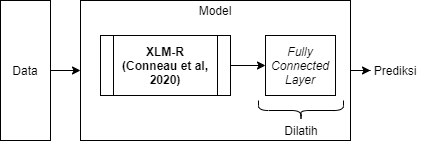
\includegraphics[width=0.75\textwidth]{resources/Head-fine-tune.png}
		\caption{ Ilustrasi \textit{fine-tuning} layer terakhir}
		\label{fig:ilustrasi_head_fine_tune}
	\end{figure}

	\begin{figure}[b]
		\centering
		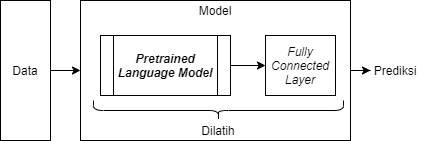
\includegraphics[width=0.75\textwidth]{resources/Full-fine-tune.png}
		\caption{ Ilustrasi \textit{fine-tuning} penuh}
		\label{fig:ilustrasi_full_fine_tune}
	\end{figure}

	\subsection{Fine-tuning}
	Untuk melakukan \textit{fine-tuning} model klasifikasi teks biner, sebuah \textit{dense layer} ditambahkan di atas keluaran dari \textit{language model} yang sudah di-\textit{pretrained}. Hal ini sama dengan teknik yang \parencite{LampleConneau2019} lakukan pada masalah klasifikasi antar bahasa dengan dataset XNLI \parencite{Conneau_Rinott_Lample_Williams_Bowman_Schwenk_Stoyanov_2018}. Penelitian, \parencite{Devlin_Chang_Lee_Toutanova_2019} mendefinisikan dua teknik \textit{fine-tuning} yang biasa dilakukan adalah melatih keseluruhan model atau hanya menggunakan \textit{language model} untuk mengekstraksi fitur dan kemudian melatih layer terakhir saja. Berikut penjelasan dan ilustrasi mengenai dua teknik tersebut
	\begin{enumerate}
		\item \textbf{Hanya Layer Terakhir}\\	
		Melatih	model secara keseluruhan memerlukan waktu dan sumber daya yang besar. Waktu dapat dipersingkat dengan membekukan dan tidak melatih lebih lanjut komponen \textit{multilingual language model} yang sudah mempelajari representasi teks antar bahasa. Komponen yang dilatih hanyalah \textit{dense layer} yang baru ditambahkan di atas model untuk melakukan klasifikasi. Ilustrasi dari proses ini dapat dilihat pada Gambar \ref{fig:ilustrasi_head_fine_tune}.

		Teknik \textit{fine-tuning} seperti ini memang menghasilkan performa yang lebih rendah dibanding melakukan \textit{fine-tuning} penuh seluruh arsitektur. Hal ini dikarenakan penggunaan representasi teks lintas bahasa yang murni dari hasil \textit{pretraining} sebagai fitur dan tidak dilakunannya penyempurnaan representasi ke permasalahan yang sedang diselesaikan. Tetapi walaupun begitu, efek dari penggunaan \textit{multilingual language model} dalam memanfaatkan bahasa yang lebih banyak sumber dayanya ke permasalahan bahasa Indonesia tetap dapat diobservasi.

		\item \textbf{Penuh}\\
		Pada teknik \textit{fine-tuning} full, seluruh arsitektur dilatih dengan fungsi \textit{loss} dari hasil klasifikasi. Dengan teknik ini, potensi secara keseluruhan dari \textit{pretrained multilingual language model} dapat diobservasi. Ilustrasi dari proses ini dapat dilihat pada Gambar \ref{fig:ilustrasi_full_fine_tune}.
		
	\end{enumerate}

	\begin{figure}[]
		\centering
		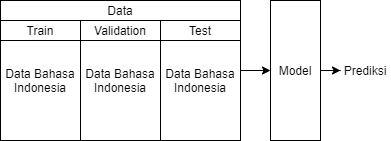
\includegraphics[width=0.75\textwidth]{resources/Data-tipe-A.png}
		\caption{Ilustrasi partisi data skenario monolingual}
		\label{fig:data_tipe_a}
	\end{figure}

	\subsection{Skenario Eksperimen}
	Terdapat tiga skenario eksperimen yang dilakukan untuk mencapai tujuan tugas akhir. Tiga skenario ini hanya memiliki perbedaan pada bahasa data yang digunakan untuk melakukan pelatihan. Berikut deskripsi tiap skenario:
	\begin{enumerate}
		\item \textbf{Skenario Monolingual}\\
		Dalam skenario ini, data untuk pelatihan, validasi, dan pengujian adalah data bahasa Indonesia. Skenario ini digunakan untuk menentukan \textit{baseline} dari performa model terhadap permasalahan. Detail ilustrasi dapat dilihat pada Gambar \ref{fig:data_tipe_a}.

		\begin{figure}[t]
		    \centering
		    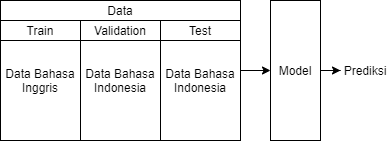
\includegraphics[width=0.75\textwidth]{resources/Data-tipe-B.png}
		    \caption{Ilustrasi partisi data skenario zero-shot}
		    \label{fig:data_tipe_b}
		\end{figure}

		\item \textbf{Skenario Zero-shot}\\
		Dalam skenario ini, data untuk pelatihan adalah data bahasa Inggris, sedangkan data validasi dan tes adalah data bahasa Indonesia. Skenario ini digunakan untuk melihat disparitas antara performa model yang dilatih dengan bahasa berbeda. Dari perbedaan performa skenario A dan B, representasi teks antar bahasa dari \textit{multilingual language model} dan juga hubungan antara dataset yang digunakan dapat dievaluasi. Detail ilustrasi dapat dilihat pada Gambar \ref{fig:data_tipe_b}.

		

		\begin{figure}[h]
		    \centering
		    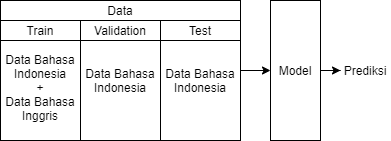
\includegraphics[width=0.75\textwidth]{resources/Data-tipe-C.png}
		    \caption{Ilustrasi partisi data skenario multilingual learning}
		    \label{fig:data_tipe_c}
		\end{figure}

		\item \textbf{Skenario Multilingual Learning}\\
		Dalam skenario ini, data untuk pelatihan adalah data bahasa Inggris dan Indonesia, sedangkan data validasi dan tes adalah data bahasa Indonesia. Pada skenario ini, perbandingan antara banyak data bahasa Inggris dengan data bahasa Indonesia divariasikan. Skenario ini digunakan untuk melihat seberapa efektif \textit{multilingual learning} dengan \textit{multilingual language model} pada klasifikasi teks bahasa Indonesia. Detail ilustrasi dapat dilihat pada Gambar \ref{fig:data_tipe_c}.
		
		
	\end{enumerate}


	